%! Author = Marjan
%! Date = 02/02/2025
% Preamble
\documentclass[a4paper, 11pt]{book}

% Packages
\usepackage{amsmath}    % For math symbols and equations
\usepackage{graphicx}   % For including graphics
\usepackage{geometry}   % For adjusting page layout
\usepackage{fancyhdr}   % For custom headers/footers
\usepackage{hyperref}   % For hyperlinks
\usepackage{listings}   % For code listing
\usepackage{lipsum}     % For placeholder text (to test layout)
\usepackage{helvet}
\usepackage{arydshln}
\usepackage{wasysym} % Helvetica as a sans-serif font alternative
\renewcommand{\rmdefault}{phv} % Set the default font family to Helvetica

% Set page margins (A4 paper)
\geometry{top=1in, bottom=1in, left=1in, right=1in}

% Set up the header
\pagestyle{fancy}
\fancyhf{}
\fancyhead[L]{System Design Notes}
\fancyhead[C]{Your Name}
\fancyhead[R]{\thepage}

% Document
\begin{document}

% Title Page
    \begin{titlepage}
        \centering
        \vspace*{2in}
        \Huge \textbf{System Design Notes}
        \vfill
        \Large Your Name
        \vfill
        \Large Date: \today
    \end{titlepage}

    \newpage

    \tableofcontents
    \newpage


    \chapter{Introduction}


    \section{Goals of this document}
    The goal of this document is to collate information that I think is useful in the area of software architecture.


    \section{OSI Model}
    Very useful when operating on different levels of abstraction in a system

    \paragraph{Level 1} - Physical

    \paragraph{Level 2} - Data link

    \paragraph{Level 3} - Network

    \paragraph{Level 4} - Transport

    \paragraph{Level 5} - Session

    \paragraph{Level 6} - Presentation

    \paragraph{Level 7} - Application


    \section{C4 Model}
    Very useful for handling different levels of abstraction

    \paragraph{Motivations: Why should I care}
    Drivers - Performance, Scalability, Fault Tolerance.
    How to measure.....latency, throughput, cost
    Consider SLA,SLO and SLI.
    Easier to code more complex stuff......


    \chapter{Gathering requirements}
    Asking is a user is not practice.
    A better and more methodical way of gethering requires ments of the desired system is through use cases and user flows.
    A use cases are a particular scenario/ situation in whcih the system is used to achieve a userss goal.
    A user flow is a more detailed step by step graphical representation of a use case.


    \section{Gathering functional requriements}
    In a formal way.
    First we need to identify all the actors or users in out system otherwise relevant usecases may not be caught.
    Second step is to describe all the possible use cases or scenarios in which an actor can use our system.
    Finally, the third step is to take each use case and expand it through a flow of events or interactions between the actor and the system.
    In each interaction we capture the action and take a note of the data that flows with it to and from the system.

    Multiple ways to represent this, one way is a sequence diagram which is a part of UML. Standard for viaualising system design.


    \section{Non functional requirements}
    These requirements have an effect on the software architecture.


    \section{Why redesign}
    System is functionally correct but speed, scalability, maintenance or security is too hard for reasons like number of users or data volume.
    System is functionally the same after redesign.
    Right architecture from the start is important
    Quality measures are used to measure how well the system performs and correlate with the architecture.
    Quality attributes have to be measurable and testable and this must be consistent.

    Something to note is that no single architecture can provide all the quality attributes. Certain attributes contradict each other.
    Some combinations are hard/ impossible to achieve.
    Tradeoffs are needed.

    Third important consideration of the system is feasibility of the quality attributes.
    Architect needs to ensure that the system is deliverable and what the client is asking for.
    Client could actually ask for something that is not technical or not technically possible.
    I.e expensive or not feasible.
    An example could be unrealistic latency expectations.
    Before approving a requirement, consulting with a domain expert to ensure that the requirement can actually be delivered.

%    Three important quality attributes when desigining a system
    \begin{itemize}
        \item Testability and measurablility
        \item Make tradeoffs between quality attributes over others
        \item Feasibility of quality attributes
    \end{itemize}


    \section{System constraints}
    Once functional requirements are defined, system function is known there are usually multiple ways to achieve the desired system
    Quality attributes will lead to tradeoffs and this is normal.
    System constraints are refered to as \quote{pillars} of an architecture.
    System constraints provide a starting point since they are usually non-negotiable and the rest of the system has to be designed around it.

    Three types

    \begin{itemize}
        \item Technical - Being locked to hardware, cloud vendors etc, must be on prem, etc.
        \item Legal - Geography, different rules in different countries where the system resides.
        \item Business - Limited budget, strict deadlines.
    \end{itemize}

    Once constraints are identified consider non-negotiable constrains and self-imposed constraints that can be removed.
    Once a set of constraints have been agreed it is hard to move away from them.
    If further in the project timeline it is found that some of those constraints were not really constraints, then the architecture will not make sense in the future.
    Another consideration is that when certain constraints are accepted, enough space needs to be left in the architecture to move away from those constraints in the future.
    Need to avoid tight coupling with certain components or constraints to allow for change otherwise whole system could be rearchitected.


    \section{Gathering System Requirements}

    \paragraph{Requirements} - Description of what we needs to be built.
    Very different when approached from a system level.
    Higher scope allows for freedom of tools and also requries a higher level of abstraction.
    Requirements are often not from an engineer or even someone technical.
    Requirements are only part of the solution.
    Client only knows the problem they need solved.
    Clarifying questions are required.

    \paragraph{Importance} - Simply build something and then fix it, wrong requirements etc, easy to fix?
    Large scale systems (i.e at this level) are big projects that cannot be changed easily.
    Many engineers involved and many hours.
    Hardware and Software costs.
    Contracts and financial obligations.
    Reputation and brand


    \section{Type of Requirements AKA Architectural Drivers}

    \paragraph{}
    Features of the System - Functional Requirements - Describe the system behaviour i.e what the system must do - Tied to the object of the system
    This doesn't determine the architecture

    \paragraph{}
    Quality Attributes - Non-functional requirements
    System properties - Scalability, Availability, Reliability, Security, Performance etc
    This does dictate the architecture

    \paragraph{}
    System Constraints - Limitations and boundaries
    Examples - Time Constraints and Deadlines, Financial Constraints, Staffing Constraints


    \chapter{Quality attributes in large scale systems}


    \section{Performance}
    Some performance metrics
    Response time - Time between client sending a request and receive a response
    Two parts, the processing time with code and databases applying business logic.
    And the \quote{waiting} time.
    The duration of time that the request or response inacitvely spends in the system.
    This time is usually spend in transit in the physical network or in software queues waiting to be handled or reach its destination.
    Waiting time is also known as latency.

    Response time can also be called end to end latency and is an importnat metric.

    Another important metric is throughput, which is the amount of data a system can process in a given interval of time.
    The more per unit of time the higher the throughput.

    \subsection{Measuring}
    Consider the end to end response time.
    Consider the distribution of response times and set a measure around it.
    Use a histogram, chart etc, statistics etc.
    Especially consider tail latency, the responses that take the most time in comparison to the rest of the values.
    This tail latency needs to be as short as possible.
    Another consideration is the performance degradation point and how fast or steep the degradation is.
    This is the point in the performance graph where the performance is starting to get significantly worse as the load increases.
    Usually this means a resource is fully utilised, could be hardware resource etc or a software queue.


    \section{Scalability}
    Load and traffic patterns never stay the same.
    Seasonal, time etc.
    Scalability is a measure of a systems ability to handle a growing amount of work in an easy and cost effective way by adding resources to the system
    Optimistic scenario is linear scalability but in practice this is hard to acheieve.
    Three ways to scale
    \begin{itemize}
        \item Horizontal scaling - Add more units of the resources that we have like multiple computers.
        Spread the load.
        No limit to scala.
        Can easily add and remove systems as required.
        Provides fault tolerance and high availability straight away.
        Not every application can support this and will require code changes.
        Changes will usually be once.
        Groups of instances require more coordination and is complex.
        \item Vertical Scaling - add more CPU, higher bandwidth etc.
        Upgrade a computer.
        No code changes required.
        This has a limit and can easily reached on a global / internet system. Easy to do with a cloud provider.
        This can centralise the system and fail to proivide fault tolerance and availability.
        \item Organisational scaling - Add more engineers.
        Before a certain point, the more engineers, the more work gets done, the more productivity is increased.
        Eventually we get less when we add too many.
        Meetings become more frequent and crowded.
        Code and merge conflicts.
        Code base will grow too large, harder for new engineers to learn the code base.
        Testing becomes hard and slow since there is no isolation, a minor change can break everything.
        Releases become risky since they include many changes.
        This impacts team scalability and engineering velocity.
    \end{itemize}
    One solution is to separate code into separate services which their own code base and tech stack, release schedule etc.

    These scalability solutions are orthogonal to each other.


    \section{Availability}
    Bad availability - Business loses money, bad things happen on important systems.
    Availability is either the fraction of time the probability that our service is operationally functional and accessible to the user.
    That time that out system is operationally functional and accessible to the user is often referred to as the uptime of the system.
    The time-out system is unavailable is referred to as downtime.
    Availability is measured as a percentage representing the ration between the uptime and the ensure time out system is running.
    This is the total sum of uptime and downtime of the system.
    Availability is measured in percentages.
    Other metrics are Mtbf and Mttr.

    Mtbf - the mean time between failures, represents the average time out system is operational.
    This is useful when dealing with multiple pieces of hardware. Most stuff is on the cloud and this avialable upfront.

    mTOR - mean time for recovery - the average time it takes to detect and recover from a failure, which is the average down time of our system.
    Until failure is recovered from the system is essentially non-operational.

    Availability of a system is the mtbf divided by the sum of mtbf and mttr.
    Use formula to estimate availability.
%    Add equation
    Note: If we minimise the average time to detect and recover from a failure theoretically all the wy to 0 we can essentially achieve 100\%
    availability regardless of the average time between failures.
    This is not practical but detectability and fast recovery has a positive impact on availability.


    \section{Fault tolerance and high availabilty}
    Three categories of failures.
    Human error, software errors like garbage collections and hardware failures.

    Best way to achieve high availability in our system is through fault tolerance.
    This enables the sytem to remain operational and available to the users despite failures within one or multiple components.
    When failure happen fault tolerance will allow the system to continue operating at the same level of performance or reduced performance.
    But it will preveitn the system from being entirely unavailable.

    Fault tolerance revolves around three major tactics.
    Failure prevention, failure detection and isolation and recovery.

    First thing to stop a system going down is to eliminate any single point of failure in our system.
    Best way to do this is through replication and redundancy.
    Replicas, spatial redundancy and time redundancy.

    Two strategies for redundancy and replication.

    \paragraph{}
    Active-active architecture - Requestions fo to all the replicas, replacement is available immediately.
    This allows for horizontal scalability but also coordination between all the replicas since they are taking requests.
    Not easy to keep in sync and has additional overhead.

    \paragraph{}
    Active-passive - one primary instance, passive instances take periodic snapshots.
    Lose ability to scale out system, all the requests go to one machine.
    Implementation is a lot easier, one instance is the most up to date, the rest or followers.

    Second tactic for fault tolerance - failure isolation and detection
    To achieve this we need a monitoring service to monitor the health of our instances via health check messages.
    Alternatively can listen to periodic messags called heartbeats, that should come periodically from healthy instances.

    In either strategy if monitoring service does not hear from the for a predefined duration of time, it can assume that the server is no longer avaiable.
    Can lead to false positives.
    Doesn't need to be perfect, as long as there are not false negatives.
    False negatives mean that the monitoring service failed since it didn't detect it.

    Monitoring service can be more complex
    Can monitor for certain conditions, can collect data like number of exceptions, latency etc.

    \subsection{Failure recovery}
    Third tactic for fault tolerance.
    If we can detect and recover from each failure faster than the user can notice then our system will have high availability.
    Once we detect the and isolate the faulty instance or server serveral actions can be taken.
    Stop sending any traffic or workload to that host.
    Attempt to restart it with the assumption that the problem will be fixed after a restart.
    Perform a rollback.
    i.e go to a previous version that was stable and correct. Useful for deploying updates.


    \section{SLA. SLO, SLI}
    Aggregates of quality attributes: SLA, SLOs and SLIs.

    \subsection{SLA}
    An agreement between the service provider and clients/users with regards to quality attributes like availabilty, performance and data durabilty and the time it takes to respond to failures.
    Includes penalties if those agreements are breached.

    Example penalties include: Refunds and service credits.

    Usually exists for external paying users but sometimes for free users.
    Occasionally for internal users but the penalties are minor if they exists.
    Free services don't usually publish SLAs.

    If other users rely on the service then it is important that they know the SLAs.
    Example users have their own SLAs

    \subsection{SLO}
    Service level objective - Individual goals that we set for the system.
    Each SLO represents a target value/ range of values that the service needs to meet.
    Quality attributes will make their way into the SLOs. Aviaabilty, end to end latency etc.

    SLOs are within a SLA.

    \subsection{SLI}
    Service level indicator - A quantitative measure of a SLO using a monitoring system. Logs could be used to calculate this.
    Once calculated this can be compared to the SL Objectives.

    \subsection{}
    SLA are usually created by business and legal teams.
    SLOs are defined by the architects and software engineers as well as the indicators.

    \paragraph{Considerations}
    Think about the metrics the user cares about.
    Don't measure everything.
    Define service level objectives around those metrics.
    From the SLO we can consider SL indicators to track the SLOs.

    Another consideration is the les SLOs the better.
    Too many SLOs make it hard for prioritisation.
    With a few SLOs its easier to focus software architecture around goals.

    Another - set realistic goals and allow room for error.
    Save costs and deal with unexpected issues.
    Commit to less than what can be provided.
    Important for external SLAs especially to avoid penalties.
    Internally these goals can be more aggressive.

    Another consideration, create a recovery plan when SLIs are indicating that SLOs are not being met.
    I.e - decide what to do if they system is down for long periods of time, performance degradation or bugs.
    This plan could include automatic alerts, automatic fail-overs, rollbacks, restarts, etc.
    and handbooks for certain situations.
    This avoids having to improvise in an emergency.


    \chapter{API Design}
    Motivations - After requirements, system can be thought of as a black box whose behaviour has a well-designed interface.
    Interface is a contract between the engineers who implement the system and the client applications who use the system.
    Such an interface is a called an API since it is going to be called by other applications remotely through a network.
    Not to be confused with programming library.
    Applications calling the Api could be front-end clients like mobiles and web browsers.
    They can be other backend systems including those from other companies.
    After internal design each component will be called by other applications within out system.

    \subsection{Category of APIs}
    Three categories of API
    \begin{itemize}
        \item Public APIs
        \item Private or Internal APIs
        \item Partner APIs
    \end{itemize}

    \subsection{Public APIs}
    Exposed to the general public and any developer can use them and call them from their application.
    Good general practice for public APIs is requiring the users to register before being allowed to send requests and use the system.
    Allows for better control over who is using the system and how they are using it.

    This in turn provides better security. Can black list users who abuse the system.

    \subsection{Private APIs}
    Only exposed internally within the company.
    Allow other teams or part of our organisation to take advantage of our system and provide value without exposing the system directly outside the organisation.

    \subsection{Partner APIs}
    Similar to public APIs but are only exposed to companies and users with a business relation ship.
    This can be in the form of buying a product or subscribing to a service.

    \paragraph{}
    Benefits of APIs is that a client can enhance their business by using the system without knowing anything about the internal design or implementation.
    Once an API is defined and exposed clients don't have to wait until the system has been finished implementing.
    Client can start making progres towards their integration with us.
    Once exposed,
    it is easier to design and architect the internal structure or out system because.
    the API essentially defines the endpoitns to the different routes in the system the user can use.

    \subsection{Desigining an API well}
    Encapsulate the internal design and implementation and abstract it away from the users/developers that want to use the system.
    Otherwise, it defeats the point of the API.
    An API needs to be completely decoupled from internal design an implementation to allow for design to change in the future, without breaking contract with the client.
    API needs to be easy to use and easy to understand, and impossible to misuse on purpose.

    This can be achieved by
    Having only one way to get certain data or perform a task rather than many.
    Having descriptive names for actions and resources, exposing only the information that the users needs and not more than that.
    Keep things consistent across our API will make using it a lot easier.
    Another good practice is keeping operations idempotent as much as possible.
    i.e an operation that doesn't have any additional effect on the result if its performed more than once.
    Idempotency is preferred since the API is going to be used over the network.
    Messages can be lost or a critical component inside out system may go down and the message was not recieved.
    Client has no idea but can resend the request with no change of effect.
    I.e same request is not processed twice.

    Another good practice is pagination.
    Used when dealing with a large payload or dataset froming part of the reqeust.
    Without it most clients will not be able to handle such a large payload or dataset and this would result in poor user experience.
    Pagination allows for the client to request only a small segment of the response by specifying the maximum size of each response from out system.
    and an offfset within the overall dataset.
    To recieve the next segment, increase the offset.

    Another good practice relates to operations that take a long time to complete.
    Asynchronous APIs.
    Client applicatoin recieves a resonse immediately without having to wait for the final result.
    The response usually includes some kind of identifier that allows the client application to track the progress and status of an operation and eventually recevie the final result.

    Very important best practice.
    Explicitly versioning an API so that the client knows which API version they are currently using.
    Motivation behind versioning APIs is to allow for non-backward compatble changes, thus allow for two versions of an API.
    Deprecate the old once gradually with good communication to the clients who are still using it.

    \paragraph{}
    APIs can be defined in any way but some best practices have emerged.


    \section{Remote Procedure Calls - RPC}
    Ability to call a client application to execute a sub routing on a remote server.
    Difference is that it looks like a remote method is being called in terms of the code the developer needs to write.
    This feature is called local transparancy. Remote or local looks the same.
    Some RPC frameworks allow for multiple programming languages so applications written in different languages can communicate.

    \subsection{How it works}
    API as well as the data types that are used in the API methods are devlaared using a special interface description language.
    This is framework / implementation specific. Effectively a schema or the communication between a remote client and a server in the system.
    After this definition using the specialised language, a code generation tool or special compiler can be used to generate two separate implementations of the API tool.
    This tool is framework specific.
    One implementation is for the client, another is for the server.
    Server side is called the server stub.
    Client side is called client stub.
    Stubs take care of all the implementation details of the remote procedure invocation.
    All custom object types that we declare using the interface description language are compiled into classes or structs depending on the language.
    Auto generate objects are refferred to as Data Transfer Objects or DTOs.

    Now at run time, wheneve rthe client appilcatoin calls that particular RPC method with some parameters the client stub takes care of coding the data.
    This is called serialization or marshalling.
    After serialisation, the connection to the remote server is inistialised and the data is send over to the stub.

    On the other end the stub is listening to the client applicatoins messags and when the message is recieved it
    unmarshalled/unserialised and then the real implementatoni of the method is invoked on the server application.

    Once the server is finished, the result is passed back through via marshalling and unmarshalling, to the client stub.
    The client application recieves the unmarshalled response as a return value.
    This will look like it was a local method call.

    Well established pattern. Frameworks, implementatoin details and performance are the only real changes.
    API developers need to pick the right framework, define the API as well as the relevant types using a RPC framework.
    The desciption then needs to be published.

    The client and server in the system are decoupled.

    When the system has been designed and implemented a stub can be generated for new clients.
    New cliets just need to generate their client stub to use the server method based on the published API definition.

    Using RPC, client and server is not restricted to programming language.

    \subsection{Pros}
    COnveinient - generate stubs which look just like local methods on objects.
    Communication details, and data passing details are abstracted away from the developers.
    Any failurres result in just exception or error depending on the programming language just like normal methods.

    \subsection{Cons}
    RPC methods are less reliable and are slower. This can lead to performance issues.
    CLient will not know how long RProcedure calls will take.

    \subsection{Considerations}
    API design will need to consider this.
    A solution is to use asynchoronous versions for slow methods which is a best practice.
    Another consideration is idempotency in the case that a message is lost/ slow

    This is geneally used when backend systems are communicated to one another but frontend systems can be considered.
    RPC is a good style when providing an API to a different company vs an end user or a webpage.
    Good for different internal components within a large scale system.

    The RPC API style is also a good way to abstract away the network communication and focus on the actions the client wants to perform on the server.

    This would be a bad fit if we want to use browser cookies or headers. There are other styles for this.
    RPC revolved more around actions rather than data and resources (Think CRUD applications).


    \begin{itemize}
        \item gRPC
        \item Apache Thirft
        \item Java Remote Method Invocation (RMI)
    \end{itemize}


    \section{Representational State Transfer - REST}
    Set of architectural constraints and best practice for web APIs. It is just a style allowing,making it easier to keep quality attributes.
    A RESTful API meets a certain traits.
    More resource orientated. Encapsulates the different entities in a system and allows for the manipulatoin of those resources through only a small number of methods.
    In a REST api a client requests a named resource and the server responds wi the current state of that resource.
    Usually done using HTTP. The resource can be implemented in a completely different way, only a representation is sent.
    Resource is just an abstraction.
    Interface is more dynamic, actions are no statically defined like in RPC.
    This is through a concept called HATEOS - hypermedia as the enginer of the application state.
    This is achieved by accompanying a state representation repsone to the client with hyper mediat links.
    The client can follow these links ad progress its interal state.

    \subsection{Achieving quality attributes}
    Important requirement of a system that provides RESTful API is that the server is stateless and does not maintain any session information about the client.
    Each message should be served by the server in isolation withouth any information about previous requests.
    This allows for high availabilty and scalability.
    If there is no session information high groups of servers can be used and the load can be spread. Client will no notice.
    Cacheability - Important requirement. This means the server either implicitly or explicitly defines each response as cacheable or non-cacheable.
    Allows the client to elimiate the potential round trip to the server and back if they response is cached somewhere closer to the client.
    This will also reduce system load.

    \subsection{Resources in RESTful APIs}
    Each resource is named and addressed usingn a URI.
    Resources are organised in a hierachy where each resource is either a simple resource or a collection resource.
    The hierachy is represented using forware slashes.
    A simple resource has a state and optionally can contain sub resorces.
    A colletion resource is a special resource that contains a list of resources of the same type.

    \subsubsection{Naming resources - best practices}
    Use nouns only. Provides distinction between actions and the resources the actions will be take on.
    Make a distinction between collection resources, and simple resources using plural and singular.
    Use clear and meaningful names. This will make the API easier to use for developers, and avoid mistakes and incorrect usages.
    Final practice. Use Unique, URL friendly names for resource identifiers for usage via the web.

    \subsection{Methods and operations}
    REST API limits the number of methods we can perform on each resource to a few predefined options.
    Creating, Updating, Deleting and getting the current state.
    When the resource is a collection resource, getting its state usually means getting a list of its sub-resources.

    Since RESTapis are commonly implemented using HTTP the operations are mapped to HTTP methods as follows.

    \begin{itemize}
        \item POST - Create an existing resource.
        \item PUT - Update an existing resource.
        \item DELETE - Delete an existing resource.
        \item GET - Get the state of an existing resource.
    \end{itemize}

    Additional can be defined but the situation is un common.

    \subsection{HTTP Semantics}
    Guarantees from HTTP semantics.
    GET is considered safe i.e it will not change the state of the resource.
    GET, PUT, DELETE are idempotent. i.e same result if you apply those operations multiple times.
    GETs are considered cacheable by default while responses to POST requests can be made cacheable by setting the approprite HTTP headers sent as part of the response to the client.
    This feature allows us to conform to the cachabilty requirements of a REST API.
    When the client needs to send additional information to the system via a POST or PUT command JSON can be used. XML is also usable.

    \subsection{Step to creating a RESTful API}
    \begin{itemize}
        \item - Identify entities in a system to serve as resources
        \item - Mapping the entities to URIs and organising the hierachy of resources based on their relationships
        \item - Choose a repsentation for each resource. Can use JSON for this and include links for HATEOS
        \item - Final step - assign HTTP methods to actions.
        \item
    \end{itemize}


    \section{GraphQL}

    
\section{GraphQL}

Dedicate this part to graphQL


    \chapter{Large Scale Systems Architectural Building Blocks}


    \section{DNS, Load Balancing, GSLB}
    Basic role, balance the traffic load amongst a group of servers in a system.
    Helps with achieve horizontal and high scalability of a system when running an application on multiple computers.
    Without a load balancer the client application will need to know the addresses of the computers hosting the application.
    This tightly couples the client application to out system's internal implementation and this makes changes hard.
    Load balancers provide an abstraction as well as avoid overloading a single server with traffic.
    This abstraction makes the application look like a single server.

    \subsection{Quality attributes from a load balancer}
    Loadbalancer provide
    High scalability -> horizontal scaling is easy
    Even easier in the cloud.

    Provides high availability. Load balancers can be configured to stop sending traffic to servers which are not healthy.

    Performance - load balancers add a little bit of latency and increase the response time but is worth the tradeoff for increased performance in terms of throughput.
    The load balancer can cater for as many backend servers as desired with some reasonsable limitations.
    Throughput is much large than what would be possible with a single server.

    Load balancer helps us achieve maintainability, since we can add, remove, upgrade servers in rotation without disrupting the client/ user.
    This would be done on a subset of the servers leaving another subset running.

    \subsection{Types of load balancers}
    DNS - internet infrastructure that maps human readable URLs to IP addresses that can be used by network routers to route to individual computers on the web.
    A single DNS record doesn't have to be mapped to a single IP address. They can be configured to return a list of IPs corresponding to different servers.
    The list returned may be in a random order.
    When recieving a list most client applications just pick the first one in the list.
    Technically this can be seen as load balancing
    Cheap and super simple but DNS doesn't know the health of servers.
    Requests may go to a down server and the DNS does't know.
    List of IP addresses changes only so often and si based on the time to live that was configured for that particular record.
    Additionallly this list of addresses that a particular domain is mapped to, can be cached in differnt locations such as the clients computer.
    That makes the time between a server going down and the point that the requests are no longer sent to that server even longer.

    Another drawback of the DNS loadbalcning strategy is that the round robin method doesn't consider the hardware resrouces of differnt servers.
    Some servers may have more powerful hardware than others, nor can it detect that one server is overloaded than others.
    Another drawback. The appliicatoins gets the IP address of all the servers, exposing implementation details whichi make the system less secure.
    Nothing stop a malvisou client application from sending requests to a single IP address in order to overload \textbf{it}

    \subsection{Addressing these drawbacks}
    Two options. Hardware load balancers and software load balancers.
    All communication between the client and servers are done via both these types of loadbalancers.
    Individual servers, and IP addressses are hidden behind the load balancer and not exposed to the users making the system more secure.

    These load balancers can peform health checks on the servers and can detect if one has became unresponsive.

    BOth can balance load more intelligently accross servers taoking into account the differnt hardware application instances are running on.

    They can be used to balance requests from users, but they can also be used inside the sytem to create an abstraction layer between services.

    Superior to DNS in terms of loadbalancing but they are usually colocated with the group of servers they balancer the load on.
    If a load balancer is too far away from the actual servers, we are adding a lot of extra latency since all communication both to and from the application has to go through the load balancer.

    When running a system in multiple geographical locations having a load balancer between them will sacrifice the performance for at least one of these locations.

    These load balancers do not support the DNS resolution, so a DNS solution will also be required.

    \subsection{Global Server Load Balancer - GSLB}
    A hybrid between a DNS service and the hardware or software load balancer.
    Typically can provide a DNS service.
    In addition it can make more intelligent routing decisions.
    On on hand, the GSLB can figure out the users location based on the origin IP inside the incoming request.
    a GSLB service has similiar monitoring capabilties to typical software or hardware loadbalancer.
    It knows the locaton and the state of each server we register with out GSLB.

    In a typical large-scale system deployment, those servers are load balancers located in differnt data centres in differnt geographical locations.
    GSLB may just return the locations of the nearest load balancer.
    The user will use that IP address from that point on to communicate with the system in that data centre through a collocated hardware or software loadbalancer.

    \subsubsection{Extra notes}
    They can be configured to route traffic on a multiple strategies. Not just geogrpahic location.
    Since they know the health of different data centres, they can route traffic based on current traffic or load on each data centre.
    Or based on estimated response time, or bandwidth between the user and that particular data centre.

    This can allow for the best performance possible for each use regardless of their geographical location.

    They are also important in disaster recovery situations. If there is an issue in one data center users can be routed to another.
    This provides high avialability.

    To prevent a load balancer from being a single point of failur, we can refister all the addresses with the GSLB DNS service or any other DNS service.
    This allows clients to get a list of all the load balancers and either pick one or send their request randomly.

    \subsection{Load Balancing Solutions}
    \begin{itemize}
        \item - HAProxy
        \item - NGINX
        \item - AWS - Application (Layer 7), Network (Layer 4), Gateway Load Balanacer, Classic Load balancer (Layer 7 and 4)
        \item - GCP %TODO add later
        \item - Azure %TODO add later
    \end{itemize}

    \subsection{GSLB Solutions}
    \begin{itemize}
        \item - Amazon Route 53
        \item - AWS Global Accelerator
        \item - GCP stuff
        \item - Azure stuff
    \end{itemize}


    \section{Message Brokers}
    A building block for asynchronous architectures.

    \subsection{Drawbacks of synchronous communitcation}
    Both applications that establish communication have to be healthy and have to remain healthy while the transaction is completed.
    Easy when the messages are short.
    Becomes more complex with larger messages.
    There is no leeway in the system to absorb spike in traffic or load.
    Horizontal scalaing is not an option since a transaction/ processing may take a long time on the system.
    The solution to this is to use a message broker.

    \subsection{What is a message broker}
    A queue data structure to store messages between senders and recievers.
    Used internally in a system, not to be exposed/interacted with by a user/client.
    Can provide additional functionality in addition to storing a buffering messages.
    Can perform message routing, transformation validation and even load balancing.
    Unlike load balancers, mesage queues decouple senders from recievers by providing their own communication protocols and APIs.
    They are a fundemntal building block in any kind of asynchronous software architecture.

    When we have two servieces communicating with eaach otehr via message broker, the sender doesn't have to wait for confirmation from the reciever after it sends the message.
    The reciver doesn't even have to be available to recieve the message when the message is sent.
    Very useful in breaking a service into multiple services.
    Another important benefit that message servies provide is buffering of messages to absorb traffic spikes.

    Many message brokers additionally off the published subscribe pattern, where multiple services can publish messages to a particular channel and multiple services can subscribe to that channel and get notrified when a new event is published.
    This makes it very easy to add services that bring in additional functionality, with out modifying the system.

    \subsection{Quality attributes from adding a message queue}
    Adds fault tolerance, since it allows different services to communicate with one another while some may be unavailable temporarily.
    Message brokers prevent messages from being lost, a characteristic of a fault tolerant system.
    This in turn helps provide higher availability for our users.
    Since a message broker can queue up messages when there is a traffic spike, it allows our suystem to scala to high traffic withouth modifying the system.

    \paragraph{Drawbacks}
    Performance - Introduces latency through the indirect communication between services. Not much of an issue in most systems.

    \subsection{Message broker solutions}
    \begin{itemize}
        \item Kafka
        \item RabitMQ
        \item AWS SQS
        \item GCP
        \item Azure %TODO add more info...?
    \end{itemize}


    \section{API Gateway}
    The problem being solved.....split the monolith in separate services....now there is a lot of service duplication and performance overhead.
    Each separate service needs to implement its own secuirty, authorisation, authentication etc....
    To solve this decouple the client application from the internal organisation of the system and simplify out external API.
    This can be done via another abstractoin called the API Gateway.
    An API Gateway is an API management service tha tsites betwen the client and the collection of backend services.
    API Gateway follows a software architectural pattern called API composition.

    In this pattern, we compose all all the different APIs of our services that we want to expose externally into a single API.
    This single API can be called by applications, by sending requests to one service. This vs sending multiple requests to different services to achieve a task.

    Provides an abstraction between the client and the rest of our system.

    \subsection{Pros}
    Allows for internal changes easily for API consumers.
    Can consolidate security issues into one place.....the API gateway.
    Bad requests get stopped at the gateway.
    Can allow a user to perform different operations depending on his permissions and role.
    Can implement rate limiting at the API Gateway to stop DDOS

    Can also improve performance of the system by saving a lot of overhead.
    Only have to do certain actions once.
    Can stop the user from making multiple requests to different places.
    This is request routing.
    With an API gateway the client makes a single request and all the backend services will have their responses aggreagatesd into a single response.

    Another performance gain is from caching certain responses for particular requests.
    Avoid making request to the backend systems.

    Another gain is monitoring and alerting is easier.
    By adding monitoring logic into the API gateway real time information can be gained on the traffic and load of they system..
    Can create alerts based on traffic variations.
    Improves observability and availability.

    Also allows for protocol translation from one place.
    Send JSON but work with RPC internally etc.
    Could communicate with legacy services the support older protocols.
    Some systems maybe reluctant to change this.
    Instead different API formats can be catered for at the API Gateway.
    I.e read some external format and translate it for the internal system.

    \subsection{Best practices and anti patterns}
    Do not include business logic here. Main purpose is API composition and routing of requests to different services.
    Those services are the ervices that make the business decisions and perform the actual tasks.
    If you add business logic to it that service will end up doing all the work. I.e a single service.
    In turn this will become an unmanagable amount of code.
    One of the problems we want to solve by splitting a service into multiple services.

    Next consideration, is that since all trafic goes through it, the API gateway may become a single point of failure.
    This can be solved by adding multiple instances of the API gateway service and placing them behind a load balancer.
    This solves scalabily, availablility and performance aspect.

    Another thing to consider is deployment. A bad release/ bug can crash the APi gateway service and the entire system can become unavailable to clients.
    Human error needs to avoided and deployments require thought.

    Additional latency is added as well since there is another service that request must go through before performing business actions.
    Avoiding the API gateways is an antipattern that should be avoided even though it may optimise the request processing.

    \subsection{API Gateway Solutions}
    \begin{itemize}
        \item Netflix Zuul (Open Source)
        \item Amazon API gateway
        \item GCP - Apigee , Google Cloud plateform API Gateway
        \item Azure
    \end{itemize}


    \section{Cloud Delivery Network Solutions and cloud}
    Can be considered to be more of a service.
    The problem being solved. Even with GSLB there still latency between the end user and the locations of the hosting server.
    Each request has to go through multiple hops over the network between different routers etc adding even more latency.
    Users will abandon a website if it takes to long to load. (Think 3 seconds plus)
    Can improve system performance etc but its content that needs to be closer to the users rather than business logic.

    \subsection{What it is}
    A globally distributed network of servers located in strategica places with the main purpose of speeding up the delivery of content to the end users.
    Solves bad user experience.
    CDNs cache website content on their servers. Referred to as edge servers. They are physically close to the user and more strategically located in terms of network infrastructure.
    Allos for the transfer of content much quicker to the user and improve the percieved system performance.
    Can be used to deliver webpage contents and assets including video streams. Both live and on demand.
    Very widely used.

    Results in faster page loads, improves system security and helps protect against DDOS since malicous requests won't go to our system.
    They will be distributed amongst a large number of servers hosted by the CDN provider.

    In addition to physical closeness, they can also be hardware optimised. I.e better hardrives, CPU etc.
    Can also reduce bandwidth by compressing content delivered over a network.
    Examples, GZIP and JavaScript minification.

    \subsection{Strategies when integrating with CDNs}
    Pull strategy - tell CDN provider which content we want on our website to be cached and how often this cache needs to be invalidated.
    This can be configured in the time to live property on each asset or type of asset.
    In this model first time a user requests a certain asset the CDN will have to populate its cache by sending a reqeust to a server in our system.
    Once that asset is cached on the CDN, subsequent reqeust by users will be served by the edge servers directly.
    This saves the network latency associated with the communication with out servers.
    When requesting an asset that has already expired, CDN will check for a new version. If it has not changed the CDN will refresh the expiry time for that asset and serve it back to the user.
    Otherwise, if a new version is avialable the CDN will receive the new version instead of the old one to the user.

    Push strategy - Manually or automatically upload or publish the content that we want deliver through a CDN.
    WHen the content changes, we are repsonsible for republishing the new versions to the edge servers.
    Some CDN providers support this model directly, other enable the strategy by setting a very long TTL for our assets so the cache never expires.
    When we want to publish a new version, we simply purge the content from the cache which forces the CDN to fetch that content from the servers whenever a user reqeusts that content.

    \subsection{Choosing the right strategy}

    \subsubsection{Advantages of pull model}
    Lower maintence on our part. Once configured which assets need to cached by the CDN and how often they need to expire nothing needs to be done to keep them up to date.
    Everything at that point will be taken care of by the CDN provider.

    \paragraph{Drawbacks}
    FIrst time there will be a longer latency as the CDN cache is popilated from the server.
    If the time to live is the same for all assets there may be freqeutn traffic spikes when those assets expire at the same time.
    This woudl result in a large number of requests from the CDN to refresh its cache at one time.

    \paragraph{}
    Add to the availability of the system but the servers still need to maintain availablity otherwise the CDN won't be able to pull the latest version of assets.

    \subsubsection{The push strategy}
    Good if the content does'nt change to frequently. Push to the CDN and then traffic will go the CDN servers.
    Will reduce traffic to out system and reduces the burden on out system to maintain high availablility.
    Even if they system goes down, users can still get data from the CDN and won't be affected by our systems internal issues at all.
    If contnet does change frequently then we have to publish new versions to the CDN otherwise users will get stale and out of data content.


    \chapter{Data storage at Scale}
    Motivations: Choosing the right databases amongst many options.


    \section{Relational Databases and ACID Transactions}

    \subsection{Relational Databases}
    Data is stored in tables.
    Each row in a table corresponds to a single record and all the records are related to each other through predefined columns they all have.
    Each column in a table has a name, a type and optionally a set of constraints .... NULL etc.
    The relatoinship between all records inside a table is what gives this type of database the name relational database.
    Strucutre of each table is decided ahead of time and is referred to as the schema of the table.
    We know what each record in the schema must have because because it is predefined.
    We can use a very robust language to query the data (analyse and update) in the table. This is SQL.
    Different implementaiton add their own features to this language. Oracle etc....
    Majority of operations are the same across all relational databases.
    Proven way of store strucutred data.
    Avoids data duplicatoin when memory is usage has to be considered (large scale)
    Use joins to combine information from multiple tables without duplication.

    \subsection{Advantages}
    Carryout complex and flexible queries using SQL. Use for analysis
    Save memory because multiple tables can be joined ..... save costs.
    Easy to reason about, very natural for humans. No sophisticated knowledge requried.
    Most importantly, provides ACID transactions.

    \begin{itemize}
        \item Atomicity
        \item Consistency
        \item Isolation
        \item Durability
    \end{itemize}

    In the context of transactions the sequence of operations should look like a single operation externally.
    Relational databases guarantee atomicity of transactions.
    Atomicity - transactions appear once or not at all.
    Consistency - guarantees that transaction that has been committed will be seen by all future queries and transactions.
    Also guarantees that data constraints that are set for the data, are met.
    Isolations - relates to concurrency, if two transactions are taking place the second transaction will not see an intermediate state. They are separate.
    Durability - once a transaction is complete its final state will persist.

    \subsection{Disadvantages}
    Rigid structure enforced by database schema enforced by the schemeas
    Schemas has to be designed ahead of time before the table can be used.
    Future changes to the schemas can lead to down time.
    Changes ideally should be avoided and not done at all.
    Through planing is required for this.
    Harder and more costly to scale because of their complexity.
    Providing SQL and ACID transactiosn is not straight forward and thus relational databases are harder to maintain.
    Due to ACID guarantess, reads are slwoer to perform compare to other types of databases.

    Differnt implementations have different performance optimisations and guarantess.

    Generally, relational databases are slower than non relational ones.

    When choosing one consider pros/cons and the use case.
    I.e is the data related, are read important.


    \section{Non-Relational Databases}
    NoSQL databases generally allow for the logical grouping or records without them having to conform to some kind of schema.
    Can easily add some kind of attributes to the different records without redesign or effecting other records.
    \textit{Most} languages do not have tables as a structure....external libraries required.
    NoSQL more typical computer science data structure (arrays, trees etc).
    This eliminates the need for object relational mappings/ ORM (Hibernate) to translate business logic for storage in a database.....

    Relational Databases are designed for efficient storage (low memory availability/ expensive memory).
    NoSQL databases are typically optimised towards faster queries.
    Different types of non-relational databases are optimised for different types of queries based on the use case.

    \paragraph{}
    Issues with flexible schemas
    Loss of ability to easily analyse those records since each record can have different structure and data.
    Joining becomes very hard, these operations are often not supported by NoSQL databases or are hard.
    Each NoSQL database supports a different set of operations and different set of datastructures.
    ACID transactions guarantees are rarely supported by non-relational databases (see exceptions).

    \paragraph{}
    Three types of NoSQL databases. Categories are somewhat blurry.

    First type is simple key, value store. We have a key that uniquely identifies a record and value that represents the data.
    The value can be anything, primitive or a binary blob.
    Can be though of as a large scale hash table/dictionary with few constraints on the type of value that can be held for each key.
    Good for caching pages or for quick fetching and ....easy.... querying.

    Second type - A document store. Collections are stored as documents. Documents have a bit more structure.
    Each document can be thought of as an object with different attributes.
    Those attributes can be different types.
    Similar to classes and fields.
    Documents are easily mapped to objects inside a programming language. Think JSON, YAML, XML

    Third Type - A graph database, an extension of a document store but with additional capabilities to traverse, link aand analyse records more efficiently.
    These types of databases are particularly optimised for navigating and analysing relationships between records in a database.

    \paragraph{Use Cases}
    Fraud detection.
    Recommendation engines.

    \subsection{When should they be used}
    Look at use case and analyse what is required from the database and what can be compromised.
    Non relation databases are better when it comes to query speed.
    Good for caching.
    Can store common query results that correspond to user views/pages.
    In memory key/value stores are optimised for this.
    Real time big data is a good use case, since relational databases are too slow and not scalable enough.
    Another use case \ldots data is not structured and different records can contain different attributes.

    Key-Value stores
    \begin{itemize}
        \item Redis
        \item Aerospike
        \item Amazon DynamoDB
    \end{itemize}
    Document Stores
    \begin{itemize}
        \item Cassandra
        \item MongoDB
    \end{itemize}
    Graph Databases
    \begin{itemize}
        \item Amazon Neptune
        \item NEO4j
    \end{itemize}


    \section{Techniques to improve performance, availability and scalbilty of databases}
    Three techniques to improve the scalability, performance and availability of a databse.

    \subsubsection{}
    Technique one - Indexing - Speeds up retrieval operations and locate the results in a sublinear time.
    Without indexing those operations could require a full table scan, which is bad for large tables.
    Example operations
    Sorting, search.
    If performed often can lead to a bottleneck

    An index is helper that we create from particular column or group of columns.
    When the index is created from a single column, the index table contains a mapping from the column value to the record that contains the value.
    Once that index table is created, we can put that table inside a data structure (good strucutres - B-Trees(or any self balancing tree), or a Hashmap).
    This will keep the values sorted and thus makes searching more efficient (think big O complexity).
    Searching is log n.
    Sorting is n log n.

    Composite indexes can be created.

    %TODO add reminder on normal form........for relational databases

    Optimising for one operation can lead to a tradeoff elsewhere.
    Indexing increases memory, decreases the speed of writes but the increases the speed of reads.
    Writing records become slower because each time a write/ new record is performed the index table must also be updated.
    Indexing is also used in non-relational databases to speed up queries.

    \subsubsection{}
    Database replication - single database, single point of failure.
    Solution, replicate data and run multiple instances of the database on different computers.
    This increases fault tolerance, availability.
    One replica goes down another can take its place and business is not effected.
    Queries can continue going to available replicas while the faulty replica is fixed.

    Get better performance and better throughput.
    Better throughput by distributing our queries across multiple computers/ replicas.

    \paragraph{Tradeoffs}
    Introduces higher complexity especially with regards to write, update and delete operations.
    (Non idempotent???)
    Making sure concurrent modifications to the same records don't conflict with each and providing predictable guarantees in terms of consistency and correctness is not a trivial task.
    Distributed databases are very hard to design, configure and manage....especially at scale.
    Requires knowledge of distributed systems....

    Database replication is widely supported by most modern databases
    Non-relation databases support replication (high availability, large scale) out of the box as they were designed with that in mind.

    Support for replication with relational databases varies amongst different implementations.

    \subsubsection{Database partioning}
    Also known as sharding.
    Split data amongst different database instances for better performance.
    Each instance will run on a different computer typically.
    More computers, more data.
    Queries which use different partitions can be done in paralell.
    We get both better performance and better availability.
    Sharing effectvely turns the database into a distributed database.
    Add complexity and overhead since routing is required for the right shard/partition as well as making sure one shard does not become too large.

    Database sharding is a common feature in most non-relational databases.
    Since by design they they decouple different records from each other.
    Storing records on different computers is a lot more natural and easier to implement.

    For relational databases, it depends on the implementation.
    Relation database queries usually involve more than one record/ are more common.
    Splitting these across multiple machines is more challenging to implement in a performant way while supporting thigns like ACID transactions or table joins.
    When choosing a relational database for high volume of data use case check for partitioning support.
    Partitioning can also be used to split infrastrcture like compute instances and redirect traffic to different machines.
    Can also do this based on mobile/browser etc running the same application.

    This routing allows for understanding which users are affected during an outage.

    \paragraph{Note}
    These three techniques are orthogonal to each other. Often used together in real user use cases.


    \section{Brewers CAP Theorem}
    %TODO find a good diagram for this

    ----- In the precesne of a network partition, a distributed database cannot guarantee both consitency and availabilty.

    The scenario of database instances not being able to communicate with one another.
    When an isolated server cannot communcate with its replicas it can either return an error or produce inconsistent data.

    Note: No network partition then no tradeoff and both consistency and availablitily can be offered.

    \begin{itemize}
        \item Consistency - Every read request received the most recent write or an error regardless of which instance is serving when considering a network partition.
        \item Availability - Every request receives a non error response without the guarantee that it contains the most recent write.
        Occasionally different clients may get a different version of a record, some may be stale but all requests return a successful value.
        \item Partition tolerance - means that the system continues to operate despite an arbitrary number of messages being delayed or lost by they network.
    \end{itemize}


    The theorem basically states one of these must be dropped when we are working with a database that may have to deal with a database partition.
    Could have a single database to guarantee consistence and availability....ie no network involved with the database....but this would not scale.
    When architecting for partition tolerance we either have to drop availability or consistency.
    Depends on the use case.

    The choice is not so distinct, more of a spectrum.
    More availability less consistency, less consistency more avialabiltiy. Depends on the tolerance requirements of the application.

    Important to get these tradeoffs in the architectural design phase, when we formalise non-functional requirements.


    \section{Scalable unstructured data storage}
%TODO where does pine cone and vector data bases fit in...........
    Unstructured data, data that doesn't follow a model or schema. Non relational data still has keys and values and structure.
    Consider binary files.
    Databases may allow for storage but they are not optimised for it.
    Limit on the object size with DBs otherwise we would encounter scalability and performance problems.
    Use cases
    - Disaster recovery
    - Archiving
    - Web hosting media like videos etc
    - Collecting data points for machine learning purposes

    Huge datasets, storage solution needs to be scalable.
    Each object can also be big.

    First solution - Distributed file system - network of storge devices
    We can get different replication consistency, and auto healing guarantees based on the file system.
    Main feature is that files are stored in a tree like structure.
    Benefit of storing unstructured data like this is that special APIs are not needed.
    Can easily modify these files.
    Performance intensive operations such as big data analysis or transformations operations on data are very fast if we do it on a distributed file system.
    ----Very useful for machine learning projects.

    Limitations of Distributed file systems
    - limited in the number of files we can create which is scalabilty issue with relatively small files like images.
    - easy access to those files via web api is hard, Additional abstractions would be required.


    Another solution - use an object store
    - A scalable storage solution designed for unstructured data at an internet scale.
    - Can scale linerly like a distributed file system by adding more storage devices.
    - Unlike a distribtued file system we have virtually no limititation on the number of binary objects we casn store in it
    - High sizes on the size of a single object....can be terrabytes.
    - Good for archiving and backups
    - Features of typical object stores can include HTTP rest API that makes them effective for storing multi media content - images etc that can be linked to a webpage
    - Object versioning is another feature, on a file system we would need to use an external versioning system.

    Differences between object store and a distributed file system.
    - No directory hierachy
    - Flat structure called buckets
    - main abstraction is an object
    - Typicall key value pairs. value being the content. Additional key value pairs exist for meta data like file type and size.
    - Objects can include an access control list who can access who has read/write permissions.
    -

    Commonly provided by cloud providers. Typicall broken into classes with each class prvoding different prices and SLA guarantess.
    Top tier is usually availbitliy of a high percentage, offers lowest latency and highest throughput
    Top tier is best for data that will be frequently accessed lke content videos, images etc.
    Middle tiers have lower guarantess for avialbitly and are cheaper.
    - These options have lmited performance and sometimes have limits frequency of usage as well.
    - Good for data backups, i.e data not needed often
    Lowest tier is good for longer term archiving. Usualy cheap and used for specific use cases.

    \subsection{Cloud vs OpenSource vs third party managed}
    Cloud may not be an option for budget, legal or performance constraints.
    There are options for on premise storage devices.
    Some follow the same APIs as some cloud vendors, so they can easily be used in hybrid cloud environments (cloud + private data centre).
    Can use the same object ID to store data in both locations.


    Just like distributed file systems, object stores use data replication although this is abstracted away.
    Ensure phyiscal storage loss will not result in loss of actual data.

    \paragraph{Object store downsides}
    Data is immutable, no edits can only be replaced with a newer version.
    Performance implications --- storing large documents that require ammends would not be feasble
    Needs a special API or a rest API unlike a distributed file system.


    Distributed systems are the preferred storage solution over object stores for high throughput solutions.

    \subsection{Scalable Unstructured Data Storage Solutions}
    Cloud based
    \begin{itemize}%TODO look into differences
        \item Amazon S3
        \item GCP
        \item Azure
        \item Alibaba
    \end{itemize}

    Open source and third party
    \begin{itemize}
        \item OpenIO - software defined
        \item MinIO - S3 and native to kubernetes
        \item Ceph - \textbf{Open-source} reliable and scalable.
    \end{itemize}


    \chapter{High-Level System Design}

    \paragraph{Software Architecture Patterns} - General repeatable solutions to commonly occurring system design problems.
    Versus design patterns which are just about organising code within a single application.
    Software architectural patterns are \quote{blueprints} for solutions that involve multiple software components.
    The purpose is to avoid repeating mistakes and antipatterns for large scale systems.

    \paragraph{Business incentives for this approach} - One - Save time and resources for devs and the organisation
    when building a solution on a similar scale.
    Use already tested development practices rather than reinvent the wheel,
    something completely new can potentially take up a lot of resources.

    \paragraph
    Two - Using an existing architecture avoids the \textit{big ball of mud}.
    The lack of structure on the system.
    In this scenario every service talks to every other service, services are tightly coupled, information is global or duplicated
    and there is no clear scope or responsibility for any of the components.

    \paragraph
    This situation can happen due to rapid growth of the company or a lack of architecture in general.

    \paragraph
    In this situation a system can be hard to develop, maintain and scale which in turn can lead to the failure of business objectives.

    \paragraph
    Third motivation - Other developers and architects can continue working on the system and can easily carry on and stick to the same architecture.
    Everyone will know the pattern that is being followed and understand what should and should not be done when adding to the system.

    \paragraph
    These are just guidelines.
    Architecture is best defined per use case / unique situation.
    As systems evolve certain patterns that were appropriate to the system in the past may not make sense anymore.
    This is normal.
    At this point some restructuring would need to be done and a migration to a different architecture pattern should be considered.

    \paragraph
    Motivations for patterns - many companies have already been through these migrations before so best practices can be adopted to make those migrations quickly and safely.

    \subsection{N/Multi-Tier Architecture}

    \paragraph{Intro}
    Organise the system into multiple physical and logical tiers.
    Logical separation limits the scope of responsibility.
    Physical tier allows each tier to be deployed, upgraded, scaled separately by different teams.

    \paragraph{}
    Note: Multi-tier and Multilayer are two different concepts.
    Multi layered architecture usually refers to the internal sepration inside a single application into multiple logical layers or modules.
    Even if the application is logically seprated into multiple layers at runtime it will run as a single unit and will be considered a single tier.

    Multi-tier architecture - applications on each tier run physically run on different infrastructure.

    \paragraph{}
    Benefits of logical and physical separation-Allows us to develop update and scale each tier independently.
    Restrictions in this architectural pattern.

    \paragraph{}
    First restriction is that each pair of applications that belong to adjacent tiers communicate with each other using the Client-server model.
    REST etc.
    Second restriction - discourages communication that skips through tiers.
    This keeps the tiers loosely coupled with each other allowing for easy changes between tiers withouth effecting the entire system.

    \paragraph{Three tier - Common variation}
    \hrule
    Top level contains UI aka presentation tier.
    Display information and take user input through a GUI\@.
    No business logic normally, this tier usually runs in the client browser.
    I.e. JavaScript etc.
    The code here should be assumed to be visible and accessible to the user.
    Bad place for business logic doing so is considered an anti-pattern.
    \hrule
    Application Tier / Business Tier/ Logic Tier.
    Provides the logic gathered from functional requirements.
    Responsible for processing the presentation tier and applying the relevant business logic to it.
    \hrule
    Data tier, this tier is responsible for storage and persistence of user and business-specific data.
    Tier may include files on a local file system or a database.

    \paragraph{Why so popular?}
    Fits a large number of use cases.
    A lot of web based services fit this model, shops, news sites etc etc.
    Very easy to scale horizontally to take large traffic volumes and handle more data.

    \paragraph{How does it scale}
    The presentation tier runs on a users device so it scales by itself....get a better phone / computer etc.
    \hrule
    Application Tier - if it is kept stateless, application instances can be kept behind a load balancer and run as many instances as we need.
    \hrule
    Database / Persistence tier - can be easily scaled if a well established distributed data base is used. DB scala - replication, partioning, sharding etc.

    \hrule
    This architectural pattern is very easy to maintain and develop because all the logic is concentrated in one place; the application tier.
    Most backend development should happen in the application tier.

    No need to worry about integration of different code bases, services or projects.

    \paragraph{Weaknesses of this pattern}

    Major drawback, the monolithic structure of the logic tier.
    Business logic should not be placed in the presentation or data tier.
    Issue is all the business logic is concentrated in a single user code base that runs as a single runtime unit.
    The implications of this, each instance of the application becomes too CPU intensive and will consume too much memory.
    This makes the application too slow and less responsive.
    This can especially be a problem with memory managed/ GC language like Java and C\# (maybe add go to this list)
    As a result applications can have longer and more frequent garbage collections.
    This can lead to requiring an upgrade of the computer the application is running on.
    Vertical scaling is both expensive and limited.

    \paragraph{}
    The second impact of the monolithic application tier is low development velocity.
    More complex code base makes it harder to develop maintian and reason about the code.
    Hiring more developers to solve this problem will not solve the problem/ add value.
    Why?
    Because more concurrent developers will simply cause more merge conflicts and higher overhead.

    \paragraph{}
    Mitigation: Could split the code into modules based on logic.
    The modules will be somewhat tightly coupled since we can release new versions of those modules only when the applications has been upgraded.
    I.e the organisational scalability of the Three-tier architecture is limited.
    Best when the code base is relatively small and not that complicated and will be maintained by a small team of developers.

    \paragraph{Examples}
    Early startups, well established companies that fit the criteria above.

    \paragraph{Variations of the Multi-Tier Architecture}
    One Tier
    Two tier - Business logic and presentation tier is combined.
    Think mobile or desktop application.
    Data tier handles persistence.

    \hrule
    More complexity - four tier.
    Between the presentation tier and the business logic tier.
    Between this tier functionality that does not belong in either can be seprated.
    Could introduce API Gateway tier that handles security,caching, data formats etc when communicating between different systems.

    \hrule
    More than four tiers is rare since they do not usually provide more value and simply adds more performance overhead.
    The source of this overhead comes from not being able to bypass tiers so as to avoid tight coupling.
    Every request would have to pass through multiple services which can increase response time/latency.
    Rarely a request would have to do so much travelling.

    \subsection{Microservices}

    \paragraph{Motivations}
    The size and complexity of the code base has grown, troubleshooting and adding new features.
    building, testing and even loading code into the IDE is now cumbersome.
    Organizationally, we now have problems.
    More developers leads to more merge conflicts, longer, larger and less productive meetings.
    At this point microservices should be considered.

    \paragraph{Microservices}
    Organises business logic as collection of loosely coupled and independently deployed services.
    Each service is owned by a small team and has a narrow scope of responsibility.

    \paragraph{Advantages}
    Codebases are now \textit{smaller} .
    Development is a lot easier and faster along with deployment and testing.
    Simply because there are fewer things.
    Code is easier to reason about and features can be added faster.
    New developers can become productive faster.
    Regarding performance and scalability, each microservice becomes less CPU intensive and takes less memory and can now run much more smoothly on commodity hardware (cloud).
    Can scala horizontally by adding more instances of low-end computers.
    Organizationally, the advantages are each service can be independently developed, maintained and deployed by a separate small team.
    This can lead to high throughput from the organisation as a whole.
    Each team can be autonomous with regard to tech stack, release schedule or process they want to follow.
    Better security in the form of fault isolation, i.e if one service starts crashing its easier to isolate and solve.

    \paragraph{Note} - Organisations can move to this architecture too quickly, without considering two factors.
    First - theoretically can achieve all those benefits from migrating to microservices, but they don't just happen and this can easily end up as a big ball of mud
    Second - microservices come with a fair amount of overhead and challenges.

    \paragraph{Pre microservices}
    To achieve full organisational decoupling so that each team can operate independently, services need to be logically seprated in way that every changed in the system can happen only in one service.
    This is to avoid involving multiple teams.
    If a change requires multiple teams then not much is gained from this migration.

    \paragraph{Microservices best practices}
    Single responsibility principle - each microservice needs to be responsible for one business cpabilyt domain resource or action.
    Monolithic API gateway can be decomposed into multiple microservices, making them more lightweight and specialised.
    Second practice is to make sure there is no coupling between different services, and this can be achieved by having a differnt database for each service.
    Note: If two services share a database then every single schema or document structure change will result in complext coordination between teams.
    If each service has its own DB then it just becomes an implementation detail that can be easily updated or replaced completly without implacting the rest of the system.

    \paragraph{Splitting the data}
    When splitting a monolithic database the data has to be split in a way that each microservice can be completely independent and fully capable of doing its work while minimising the need to call other services.
    Data duplication is expected and is normal in this scenario.
    Duplication is a tradeoff here and an overhead of using this architecture.

    Following best practices will help achieve a positive outcome when moving to microservices.

    \paragraph{Practical note}
    Microservices brings in additional complexity and overhead.
    This only brings business value when the system reaches a certain size and the organisation is of a certain scale.
    Start with a monolith approach first.
    When that is no longer working for the use case, then move to micro services.

    \paragraph{Conclusion}

    The benefits of microservices architecture.
    Higher organisational and operation scalability, better performance, faster development, better security.
    Best practices are required to realise these advantages and are only really applicable to systems and organisations of a certain size.

    \subsection{Event-Driven Architecture}

    \paragraph{Motivation}
    If microservice A want to communicate with Microservice B, then not only does it require awareness of service B, it also needs to know how to call what API microservice B provides and how to call it at run time.
    Also, microservice A has to call microservice B synchronously and wait for its response (No always async etc????).
    Microservice A has a dependency on microservice B\@.

    \paragraph
    In an event driven architecture, instead of direct messages that issue commands or request that ask for data, we have only events.
    An event is an immutable statement of a fact or a change.
    In an Event-Driven architecture we have three components.
    Sending side - We have event emitters, which are also referred to as producers.
    Receiving side - We have event consumers
    And inbetween we have the event channel (a message broker), Kafka?

    \paragraph{Advantages}
    When we use the Event-Driven Architecture style with microservices we can get a lot of benefits.
    Now the dependency between Microservice A and B is removed.
    Microservice A doesn't need to know anything about the existence of microservice B
    And once microservice A produces the event, it doesn't need to wait for any response from any consumer.
    Because services don't need to know about each other's existence or API and all the messages are exchanged completely asynchronously, we can decouple microservices more effectively.
    This results in higher scalability.
    More services or integrations can be added to to the system without making any changes.
    Horizontal and organisational scalability is achieved via EDA.
    This architecture also allows us to analyse streams of data, detect patterns and act up on them in real time.

    \paragraph{Further advantages}
    When all events that occur in a system are stored in a message broker, in addition to data analysis an very powerful architecture pattern can be implemented.
    This is called event sourcing.
    By using event sourcing events can be replayed to identify the current state of a system rather than saving the state in a database.
    Because events are immutable we're never modifying them.
    We simply append new events to the log as they come.
    Using event sourcing we can store events for as long as we want.
    Querying can be made faster by adding snapshot events.

    \paragraph{CQRS}
    Another architectural pattern that can be implemented as a result of EDA
    Command query responsibility segregation.
    This solves two problems.

    First problem is optimizing a database that has a high read and update operations.
    In this scenario concurrent operations to the same record or tables contend with each other making the system slow.
    Additionally, if we use a distributed database, generally we can optimize it for one type of operation at the expense of teh other.
    (Cap theorem?)
    Ad-hoc solution - We can optimize one operation at the expense of the other when an application is read/write heavy.
    However, when the both operations are equally important we have a problem.
    CQRS architectural pattern allows us to separate Update and Read operations into separate databases, sitting behind separate services.
    In this case service A would take all the update operations and perform them in their own database, where it optimally stores the data for such updates.
    Additionally, every time an update operation is performed if publishes an event into a message broker.
    Meanwhile, service B will subscribe to those update events and applies those changes in its own read optimised database and now all read operations will go to service B.
    Both update and read operations can go to separate services without any contention/interference.

    Further, the data can be optimized for each type of operation.


    The second problem that CQRS helps solve is joining multiple tables that are located in separate databases that belong to two different microservices.
    Prior to monoliths all data was in one table.
    If that was a relational database all the records could be joined and then analysed.
    Post microservices, this is not the case assuming that best practice has been followed.
    Joins are harder now.
    Requests need to be sent to each service separately which is slower.
    This data needs to be combined programmatically because now we potentially have different types of databases.
    Some of these databases may not even be relational.


    CQRS solves this problem.
    Every time there is a change of data in a services database, those services would publish those changes as an event to which other services subscribe to.
    The other service will store what is called a materialized view of the joined read-to-query data from both service A and service B in its own read-only database.
    Whenever we need to get a join view we can just send a request to the joining service rather than send a request to two services.

    \paragraph{summary of EDA}
    When combined with microservices this allows for decoupling of services potentially allowing for horizontal and organiszation scalability.
    Event driven architecture allows us to analyse and respond to large streams of data in real time.

    \paragraph{Pattern within EDA}
    Event sourcing - allows for the auditing and storage of the current state of a business entity by only appending events and replaying them when needed.
    CQRS - Allows for database optimisation for both updates and reads by splitting the operations into separate services.
    This allows for the efficient joining of data from separate services.

    \chapter{Microservices in depth}

    \section{Migration to microservices architecture}
    \section{Principles and Best Practices}
    \section{Event driven architecture}
    \section{Event driven microservices}
    \section{Testing Microservices and Event-Driven Architecture}
    \section{Observability in Microservices Architecture}
    \section{Deployment of Microservices and Event-Driven Architecture in Production}

    \chapter{Cloud Architecure patterns}

    \section{Scalabilty patterns}
    \section{Performance Patterns for Data Intensive Systems}
    \section{Software Extensibility Architecure Patterns}
    \section{Reliability, Error Handling and Recovery Software Architecture Patterns}
    \section{Deployment and Production Testing Patterns}

    \paragraph{Note} EDA and Microservices aren't a requirement for each other but they are commonly used together to achieve greater decoupling.
    Issues to address with Microservices, organisational scaling and technical problems relating to scaling.
    Refactoring is harder and application becomes less stable, small issues can jeopardise the whole system.
    Solution, organise business logic as loosely coupled deployable independently deployable services.
    Each service is owned by a small team and has narrow scope of responsibility.
    Now we have organisational scalability, building is faster, less burden on the developer, each binary is smaller in size.
    Testing and reasoning is easier, onboarding is faster and this development velocity is faster.
    Hardware demands are easier since commodity hardware can now be used due to less CPU and memory usage.
    Flexible tool choice for development teams.
    Refactoring is easier.
    Higher system stability, the damage caused by a bug etc is much smaller since each service is deployed separately.

    \paragraph{Barriers to implementing microservices}
    Method calls have now become network calls between different computers bringing in latency issues.
    In distributed systems each component is unreliable.
    Although testing is faster no guarantee all the services will work when deployed together.
    This can lead to complicated integration tests than can impact prodictivity.
    Would be hard to understand which team owns the integration tests.
    Fixing bugs and troubleshooting performance is much harder in microservies
    Incorrect scope identification for a service can also cause additional organiszatoinal overhead.
    Could lead to duplicated effort.


    \chapter{Big Data Architeciture}

    \paragraph{Terminology} - Data sets which are too big or too complex or are produced at too fast that exceed the capacity of a traditional application.
    Characteristics are typically volume, variety, rate/velocity.
    This data can be used to gain insights/conclusions via visualisation, querying or predictive analysis.
    Can also be used to find anomalies, analysing logs.


    \section{Batch}
    requires the storage of incoming data in a distributed database or a distributed files system.
    Data is never modified, it is only added to the end.
    Key principal is that the data is processed in batches or records on a fixed schedule, or a fixed number of records that we want to process.
    The schedule can be adapted for the users/clients needs.
    Each time a batch processing job runs in can process new data and produce and up-to-date view of all the current data.
    This can be stored in a well-structured and indexed database that can be queried to get insights.
    Could analyse recent data or the whole data set.

    This data is not processed in real time.

    Note: This data can be used to create a Machine learning model.

    Batch processing provides the user with high availability, no downtime for users the old data view is still available.

    Batch processing is more efficient vs processing each piece of data individually. Also higher tolerance towards human error, with regards to bad code/ deployment issues.
    Batch processing can be used to perform complex data analysis of large data sets.....

    \paragraph{Drawbacks}
    Long delay between data coming in and the result we get from the processing job.
    The view is not real time which can be an issue in some use cases (Trading, 24/7 systems etc).
    Forces users to wait a long time before they can act on the insights from the system.
    May not know that the data is not in real time.


    \section{Real time processing / Streaming}
    Each new event into the system is placed into a queue or a message broker, on the other end there is a processing job that processes each bit of data as it comes through.
    After processing the processing job updates the database that provides querying capabilities for real time visualisation and analysis.

    \paragraph{Pros}
    Can respond to data immediately

    \paragraph{Cons}
    Hard to do any complex analysis in real time as a result insight may be poor compared to to batch.
    Hard to data fusion in real time, at different time points or analysing historic data. Only limited to recent data for predictions.


    \section{Lambda architecture}
    May need processes of both strategies.
    Lambda architecture takes advantages of both.
    Aims to find the balance between fault tolerance and comprehensive analysis of the data from batch processing and the low latency that we get from real time.

    In this architecture the infrastructure is divided into three layers, batch, speed, and serving layer.

    Data that enters the system is dispatched into both the batch layer and the speed layer simultaneously.
    The purpose of the batch layer is to manage out data set and be the system of records.
    The data in our master set is immutable and new data is appended, never modified.
    This data is usually on a distributed files system, optimized for storing big files containing massive amountds of data.
    The second purpose of the batch layer is to pre computer our batch views.
    Every time we run out batch processing job, it processes all the data that we have in out master data set. Once the processing is cimplete it indexes and store the data in a read only database.
    Typically, this overrides the existing pre computed views that we created the previous time we ran the processing job.
    Note: The batch layer aims at perfect accuracy and operates on the entire data set.

    \paragraph{Speed Layer}
    Data is sent to this layer in parallel.
    Real time strategy is used here.
    All the data goes into a queue or a message broker and is then picked up as it arrives by the processing job.
    Processing job analyses the new even and adds the processed even to the real time view ready for querying.
    This layer compensates for the latency in the batch layer.
    Unlike the batch layer it only operates on the most recent data and doesn't attempt to provied a cimplete view or make any data corrections.

    This layer exists between the last time a batch was run and the present moment/recent data.

    \paragraph{Serving layer}
    The serving layers purpose is to respond to queries and merge the data from both the batch and speed layer and update the real time views.


    \chapter{Components}

    \subsection{Load balancing}

    \subsection{Message Brokers}

    \subsubsection{Kafka}

    \subsection{API Design}

    \subsubsection{REST}

    \subsubsection{GraphQL}

    \subsubsection{RPC}

    \subsection{Data Storage}

    \subsubsection{CDN}

    \subsection{Design Patterns}

    \subsubsection{Scalability}

    \paragraph{Load Balancing}

    \paragraph{Pipes and filters}

    \paragraph{Scatter and Gather}

    \subsubsection{Microservices specific}

    \paragraph{Execution orchestrator}

    \paragraph{Choreography}

    \subsubsection{Extensibility}

    \paragraph{Sidecar}

    \paragraph{Adapters}

    \paragraph{Frontends for Backends}

    \subsubsection{Availablility, error handling and recovery}

    \paragraph{Rate Limiting}

    \paragraph{Retry Pattern}

    \paragraph{Circuit breaker}

    \paragraph{Dead Letter Queue}

    \subsection{Data intensive applications patterns}

    \subsubsection{Map Reduce}

    \subsubsection{Saga}

    \subsubsection{Transactional Outbox}

    \subsubsection{Materialized View Pattern}

    \subsubsection{CQRS}

    \subsubsection{Event Sourcing}


    \section{Detailed Design}

    \subsection{Caching}
    Redis

    \subsection{Queues}
    Kafka

    \subsection{Protocols}

    \subsubsection{TCP}

    \subsubsection{UDP}

    \subsection{Threads and Concurrency}

    \paragraph{Actor model and Akka}
    Java low level and higher level

    \paragraph{Functional}
    Scala.....

    \paragraph{Application level}
    Scaling via instances


    \chapter{Databases}

    \paragraph{NoSQL}
    MongoDB.....graph databases

    \paragraph{SQL}

    \subsection{Networks}


    \section{Performance and Scalability}

    \subsection{Testing}

    \paragraph{Gatling}

    \paragraph{Code performance}
    Hmmmm maybe JVM specific here


    \section{Distributed Systems}

    \subsection{Clusters}
    Kubernetes

    \subsection{Storage}


    \chapter{Performance}


    \chapter{Scalability}


    \chapter{Reliability}


    \chapter{Tech stacks}


    \chapter{Deployments}
    Docker, Jenkins


    \chapter{System design security concerns}


    \section{Introduction}
    Cover security from a system design point of view.


    \section{Network security}


    \section{Encryption}


    \section{Digital signatures}


    \section{Authentication}


    \chapter{Useful resources}
    Stuff used to create these notes

    https://www.udemy.com/course/software-architecture-design-of-modern-large-scale-systems
    https://www.udemy.com/course/the-complete-microservices-event-driven-architecture

    \newpage

% Example of including a code snippet


    \section{Code Example}
    \begin{lstlisting}[language=Java, caption=Java Code for a Simple Cache]
public class SimpleCache {
    private Map<String, String> cache = new HashMap<>();

    public String get(String key) {
        return cache.get(key);
    }

    public void put(String key, String value) {
        cache.put(key, value);
    }
}
    \end{lstlisting}


    \chapter{Diagrams}

    \begin{figure}[h]
        \centering
        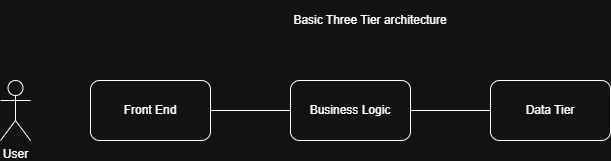
\includegraphics[width=0.8\textwidth]{basic-architecture} % Change to your filename
        \caption{Three tier architecture}
        \label{fig:drawio-diagram}
    \end{figure}


    \chapter{Architecture examples}


\end{document}
